\documentclass[tikz]{standalone}
\input{common/tikzBase}
\usetikzlibrary{}
\lstset{
    language=C,
    morekeywords=item,
    style=smaller,
    moredelim={**[is][\btHL<2>]{~2~}{~end~}},
}
\newsavebox{\overExampleACode}
\begin{document}
\begin{lrbox}{\overExampleACode}
\begin{lstlisting}
item *load_items(int len) {
  int total_size = ~2~len * sizeof(item);~end~
  if (total_size >= LIMIT) {
    return NULL;
  }
  item *items = malloc(total_size);
  for (int i = 0; i < len; ++i) {
    int failed = read_item(&items[i]);
    if (failed) {
      free(items);
      return NULL;
    }
  }
  return items;
}
\end{lstlisting}
\end{lrbox}

\setSlide{1}
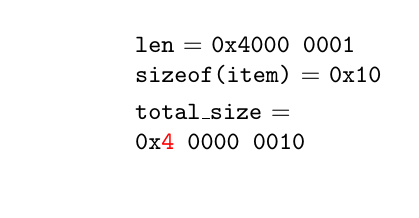
\begin{tikzpicture}
\node[anchor=north east] (code) at (-1,0) {
\usebox{\overExampleACode}
};
\node[align=left,anchor=north west,font=\small] (t1) at (0,0) {
    {\tt len} = {\tt 0x4000 0001} \\
    {\tt sizeof(item)} = {\tt 0x10}
};
\node[align=left,anchor=north west,font=\small] (t2) at (t1.south west) {
    {\tt total\_size} = \\
    {\tt 0x\textcolor{red}{4} 0000 0010} \\
};
\end{tikzpicture}
\end{document}
